\section{Case-study : using MLOps to improve NACE classification}
\label{sec:mlops}

This chapter aims, through a concrete example, to illustrate how Insee managed to deploy its first machine learning (ML) model into production. It will provide an in-depth description of the MLOps approach that this project strived to adhere to, focusing on the various technologies that were employed. In particular, we will highlight how cloud technologies were instrumental in building a solution iteratively and how Onyxia greatly facilitated this process by providing flexible development environments as well as tools to deploy and monitor models, promoting a continuous improvement loop. The entire project is available in open source\footnote{\url{https://github.com/orgs/InseeFrLab/teams/codification-ape/repositories}} and remains under active development.






\subsection{Improving the NACE classification process using ML methods}

\subsubsection{Motivation}

Coding tasks are common operations for NSOs and can sometimes be challenging due to the size of nomenclatures. At Insee, a sophisticated coding tool called Sicore was developed in the 1990s to perform various classification tasks. It consists in a coding engine containing a large number of deterministic rules which identify ground-truth labels. Each input label goes through these rules and when a ground-truth label is recognized, the associated code is assigned. When the label is not recognized, it must be manually classified by an Insee agent. 

Two main reasons drove the experimentation of new coding methods. Firstly, there was an internal change with the redesign of the Sirene registry, which lists all companies in France and assigns them a unique identifier, the Siren number, used by public institutions. The main goals of this revamping were to improve the daily management of the registry for Insee agents and to reduce waiting times for companies. Additionally, at the national level, the government launched a one-stop shop for business formalities, allowing more flexibility for business owners in describing their main activities. Initial testing exercises revealed that Sicore was no longer the suitable tool for performing NACE classification, as only 30\% of the input data were being automatically coded.

Three stakeholders were involved in this project: the \textit{business team}\footnote{We refer to the business team, the team that has business knowledge i.e. who knows the NACE perfectly.} responsible for managing the Sirene registry, the \textit{IT team} developing software related to the registry's operation, and the \textit{innovation team} responsible for implementing the new coding tool. The latter team is the Insee Lab, which was created in 2017 with the objective of providing support to other teams on innovation topics to streamline their various projects.

\subsubsection{Classification task}

The project we are describing consists in a standard NLP classification problem. Starting from a textual description of the activity, we want to predict the associated class in the NACE Rev. 2 nomenclature. This nomenclature has the particularity of being hierarchical and contains 5 different levels\footnote{Actually, there are 5 different levels in France but only 4 at the European level.}: section, division, group, class, and subclass. In total, 732 subclasses are included in the nomenclature, which is the level at which we aim to perform the classification. Table \ref{tab:nace-nomenclature} provides an example of this hierarchical structure.

\begin{table}[htbp]
    \centering
    \begin{tabular}{llll}
    \textbf{Level} & \textbf{NACE} & \textbf{Title} & \textbf{Size} \\ \hline
    Section & H & Transportation and storage & 21 \\ \hline
    Division & 52 & Warehousing and support activities for transportation & 88 \\ \hline
    Group & 522 & Support activities for transportation & 272 \\ \hline
    Class & 5224 & Cargo handling & 615 \\ \hline
    \textbf{Subclass} & \textbf{\textcolor{red}{5224A}} & \textbf{Harbour handling} & \textbf{\textcolor{red}{732}} \\ 
    \end{tabular}
    \caption{NACE Nomenclature}
    \label{tab:nace-nomenclature}
    \end{table}

With the establishment of the one-stop shop, business owners now describe their activity description with a free-text field. As a result, the new labels are very different from the harmonized labels that were previously received. Therefore, it was decided to work with ML models, that are known to be effective on supervised text classification tasks \cite{li2022survey}. This represents a significant paradigm shift from Insee's perspective, as ML was not traditionally used in the actual production of official statistics. Besides, the perspective of putting the new model in production was considered from the outset, guiding numerous methodological and technical choices. As such, several strategic choices had to be made from the outset, including the methodology, the choice of a development environment consistent with the target production environment, and the adoption of collaborative work methods.

\subsubsection{Methodology}

Text classification from the free-text field provided by business owners is a complex task: the activity descriptions are relatively short and thus contain limited statistical information, can contain spelling mistakes, and often require domain knowledge to be properly classified. On such task, traditional text analysis methods such as count vectorization or TF-IDF often fall short whereas neural-network-based embedding methods tend to perform better \cite{li2022survey}. However, such architectures impose greater demands on the production setting, as they are much larger and often require specific hardware such as GPUs to be fine-tuned and perform inference with acceptable latency. These constraints led us away from the most powerful language models, such as Transformer models, and instead directed us towards the fastText model \cite{joulin2016bag}, a simpler embedding-based classifier. The fastText model is extremely fast to train, even from scratch, and inference doesn't require a GPU to achieve low latency time. Besides, the model yielded excellent performance results for our use-case which, considering the time and human resource constraints, were more than sufficient to enhance the existing process. Finally, the model's architecture is relatively simple, which simplified communication and adoption within the various Insee teams.

The fastText model relies on a bag-of-words model to obtain embeddings and a classification layer based on logistic regression. The bag-of-words approach involves representing a text as the set of vector representations of each of its constituent tokens. With FastText, the embedding of a sentence is computed as a function of the individual embeddings, typically the average. In the case of supervised text classification, the embedding matrix and the classifier's parameters are learned simultaneously during training by gradient descent, minimizing the cross-entropy loss function. The specificity of the fastText model compared to other embeddings-based approaches is that embeddings are not only computed on words but also on word n-grams and character n-grams, providing more context and reducing biases due to spelling mistakes. Figure \ref{fig:fasttext} represents the full pipeline of operations performed by fastText on an example text input.

\begin{figure}[htbp]
    \centering
    \makebox[\textwidth][c]{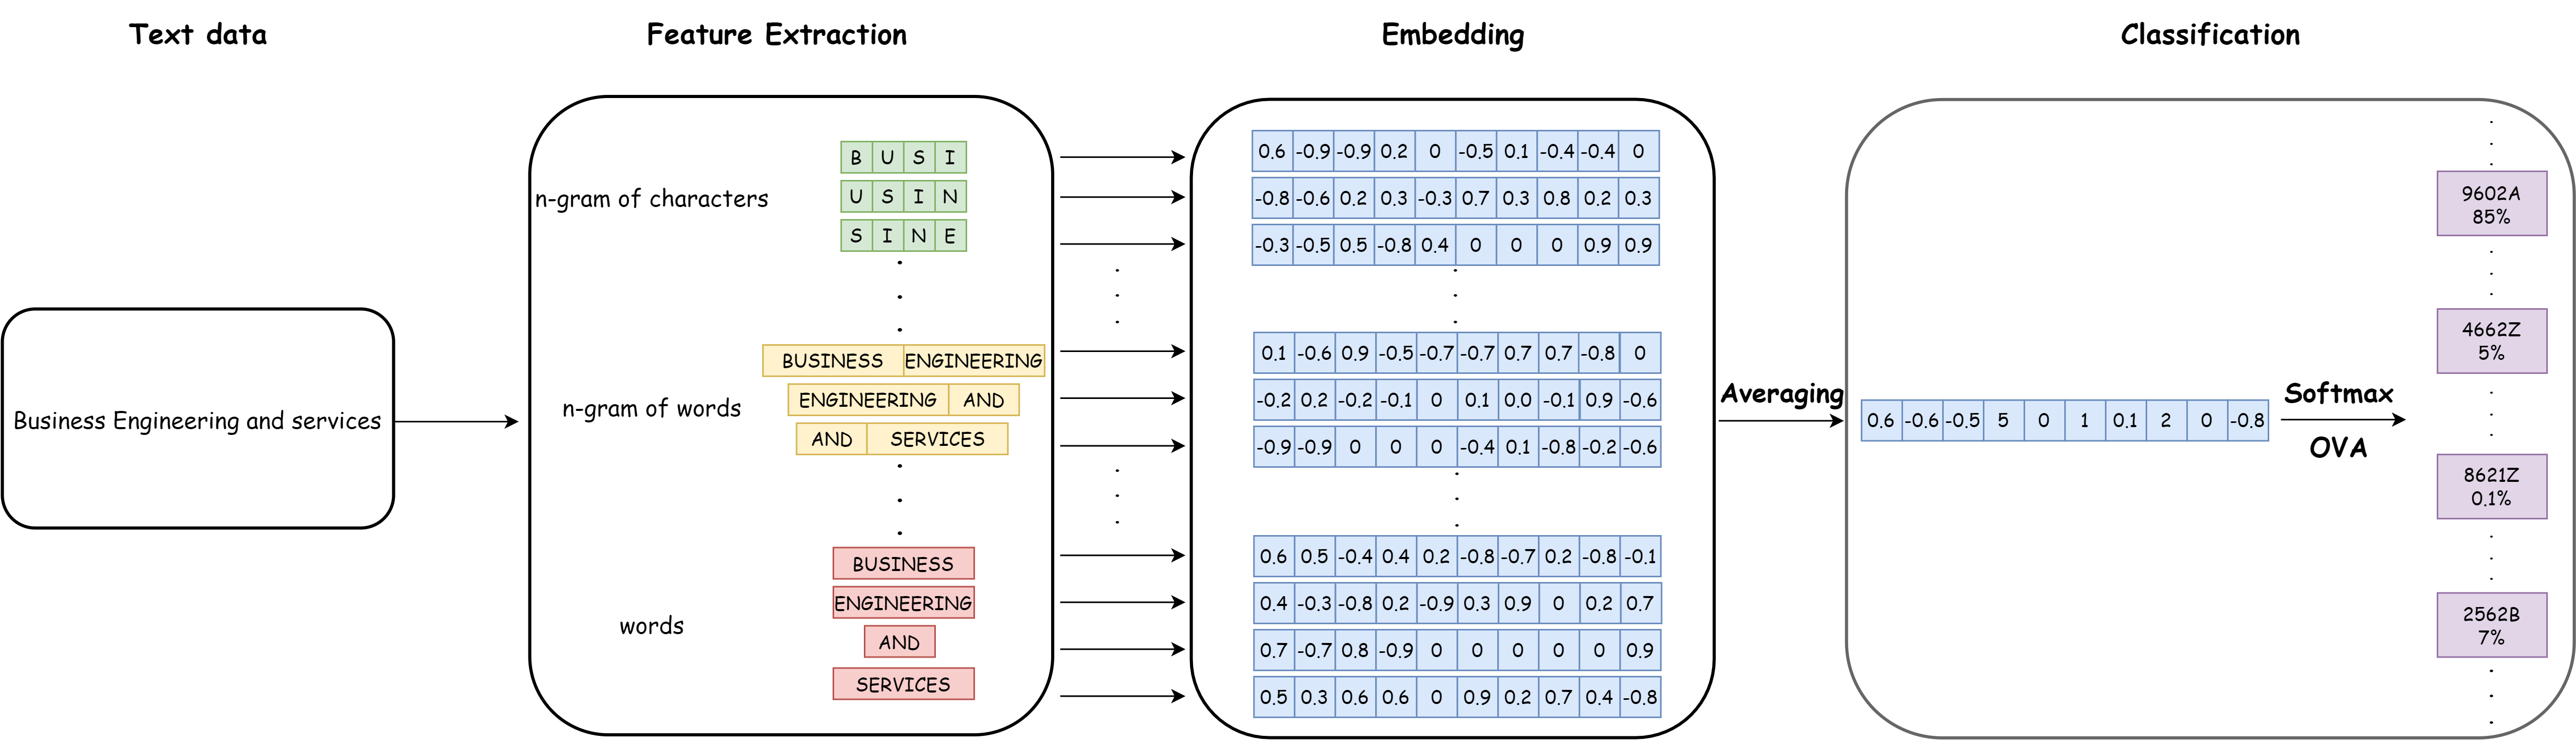
\includegraphics[width=1.5\textwidth]{sections/img/fasttext.png}}
    \caption{Simplified architecture of the fastText model}
    \label{fig:fasttext}
\end{figure}






\subsection{A production-first approach with MLOps}

From the very onset of this project, the target was to go beyond mere experimentation and put the model in production. Besides, the goal with this pilot project was also to build a template for future ML projects at Insee. We thus strove to enforce best development practices from the very beginning of the project: following community standards for code quality, using scripts-based development over notebooks, building a modular package-like structure, etc. However, compared to traditional development projects, machine learning projects have specific features that make it necessary to apply a complementary set of best practices, gathered under the name of MLOps.

\subsubsection{From DevOps to MLOps}
\label{subsubsec:devops-mlops}

DevOps is a set of practices designed to foster collaboration between development (Dev) and operations (Ops) teams. The fundamental idea is to integrate the full lifecycle of a project in a single automated continuum. An important tool to achieve this continuity is CI/CD pipelines. With continuous integration (CI), each commit of new source code will trigger a pipeline of standardized operations, such as building the application, testing it and making it available as a release. Then, continuous deployment (CD) consists in tools to automate the deployment of the new code and limit manual intervention, while ensuring proper monitoring to guarantee process stability and security. This approach promotes a more rapid, continual release of necessary feature changes or additions. Furthermore, by encouraging collaboration between teams, DevOps also promotes a quicker cycle of innovation, allowing teams to address issues as they arise and incorporate feedback effectively throughout the project lifecycle.

The MLOps approach can be seen as an extension of DevOps, developed to address the specific challenges related to managing the lifecycle of ML models. Fundamentally, both DevOps and MLOps aim at building software in a more automated and robust manner. The main difference is that in MLOps, this software also has a machine learning component. Consequently, the lifecycle of the project gets more complex. The underlying ML model needs to be trained, often periodically in order to prevent potential performance losses over time. Data ingestion must also be included in the pipeline, as new data may be used to improve performance. Figure~\ref{fig:mlops-cycle} presents the steps of a ML project using the continuous representation traditionally seen in DevOps. This illustrates a fundamental principle of MLOps, the need for continuous improvement, described in more details in section~\ref{sec:principles-mlops}.

\begin{figure}[htbp]
    \centering
    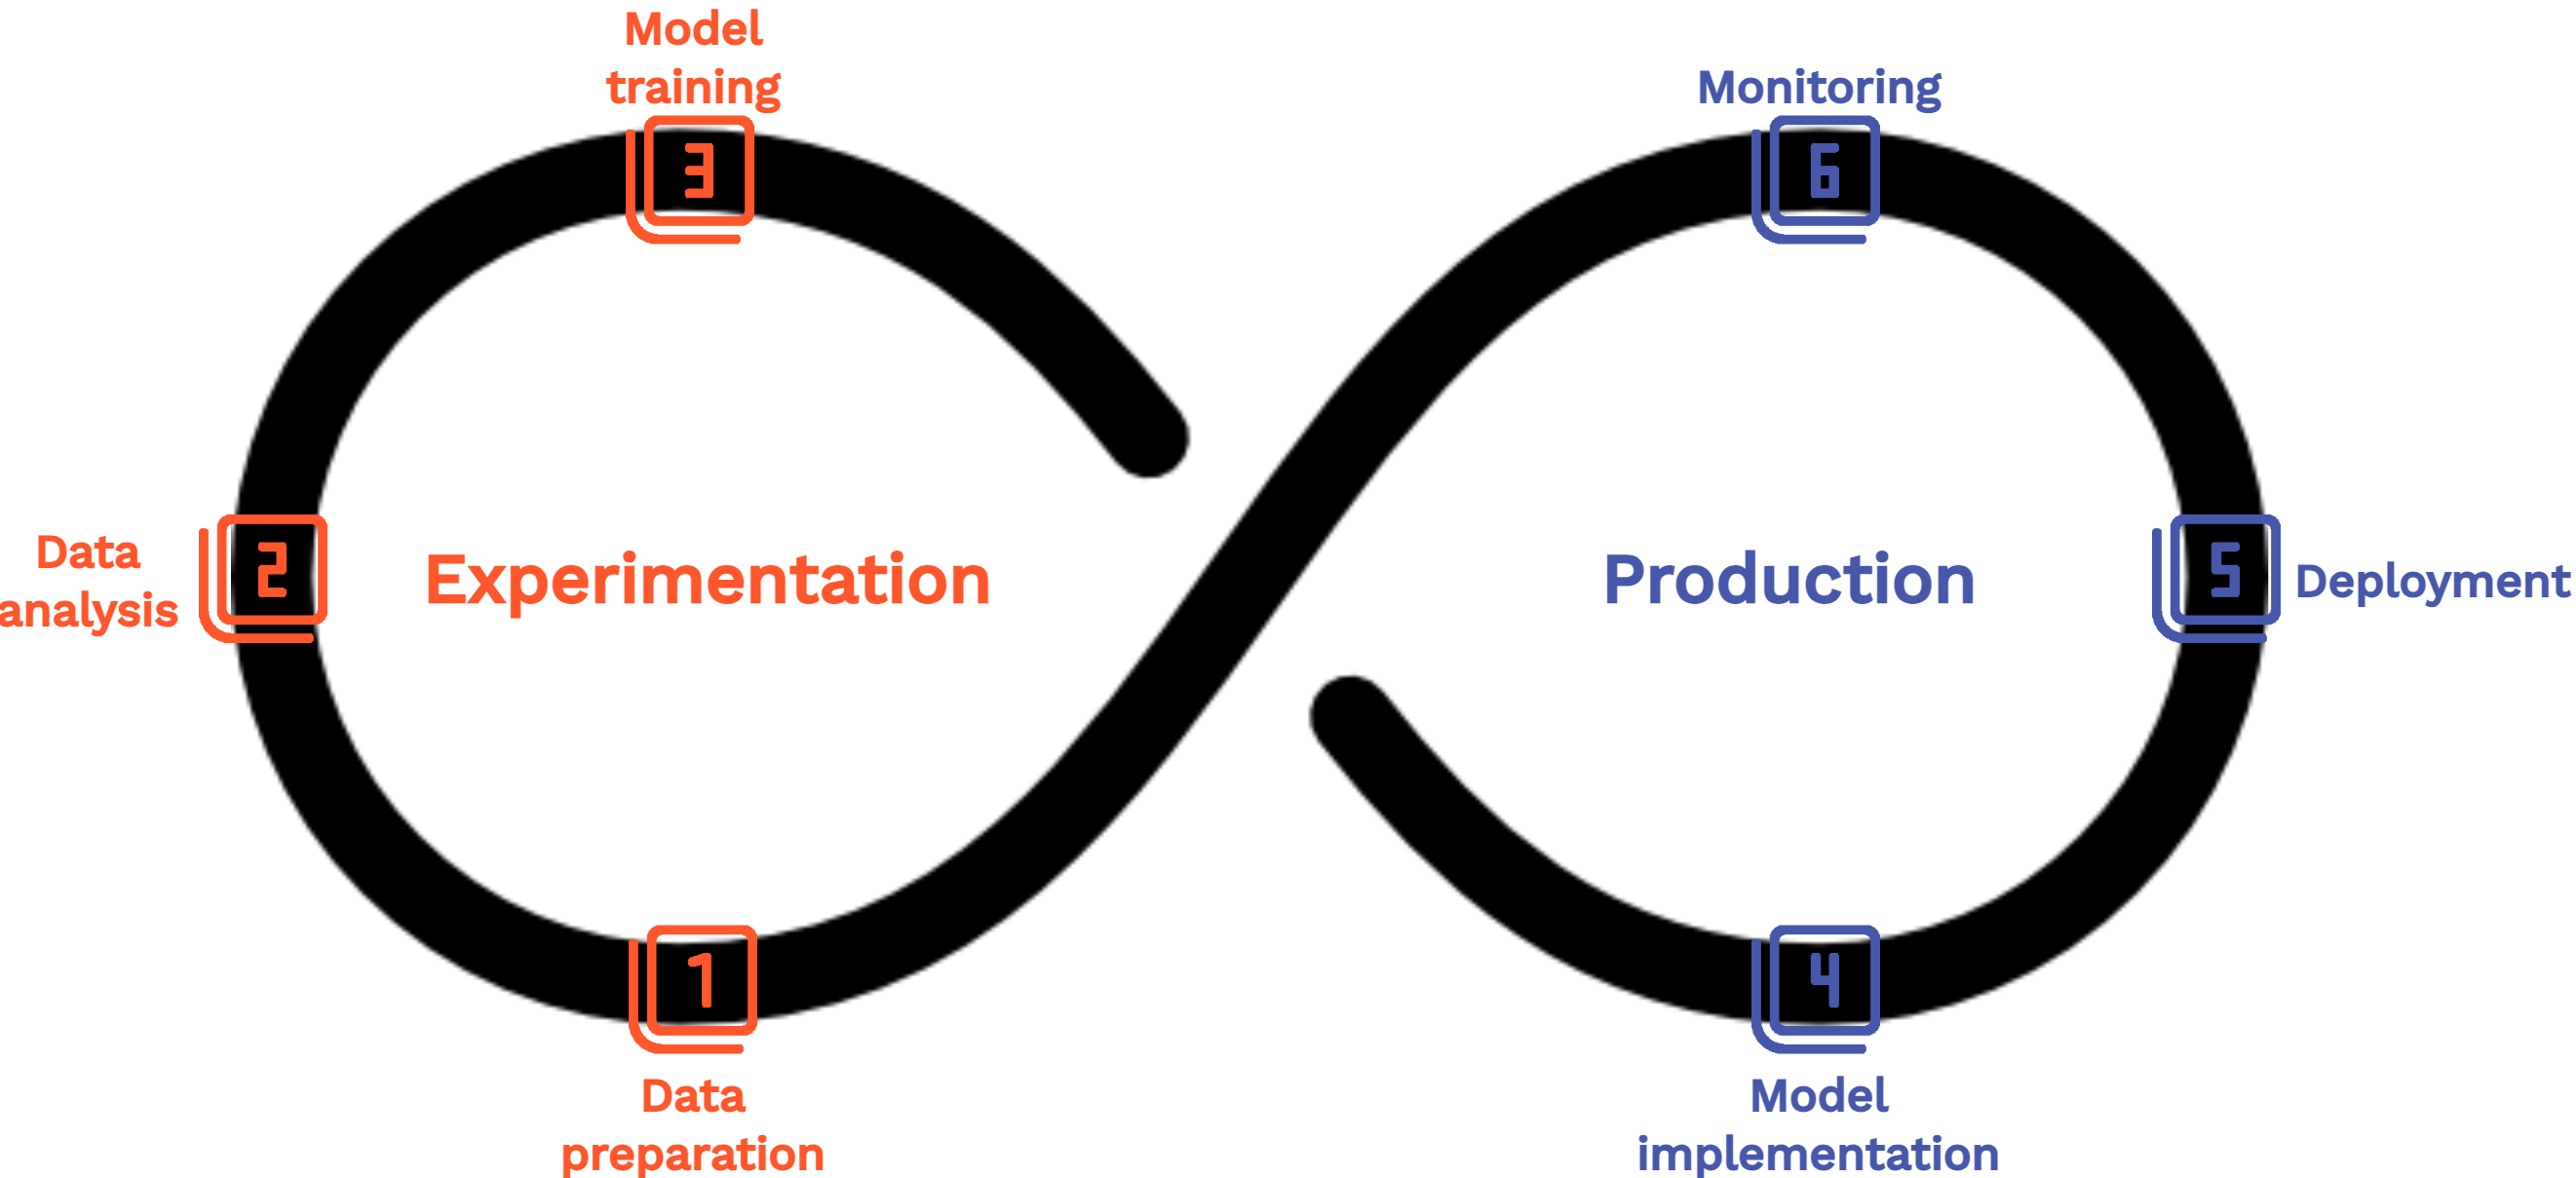
\includegraphics[width=\textwidth]{sections/img/mlops-cycle.png}
    \caption{The MLOps approach promotes a continuous management of ML projects lifecycle}
    \label{fig:mlops-cycle}
\end{figure}

\subsubsection{Principles of MLOps}
\label{sec:principles-mlops}

MLOps is defined by a few core principles that are crucial for building production-ready and scalable ML applications. These principles are designed to address the specific challenges associated with ML workflows.

The most fundamental principle of MLOps is continuous improvement, in order to reflect the iterative nature of ML projects. In the experimentation phase, the model is developed using a training dataset, which will generally differ somewhat from the target data. When a model is deployed in production, the new data that the model needs to perform prediction one can reveal insights about the model's performance and potential shortcomings. These insights necessitate a return to the experimentation phase, where data scientists adjust or redesign their models to address any discovered issues or to improve accuracy. This principle thus emphasizes the importance of building a feedback loop that enables ongoing enhancements throughout the lifecycle of a model. Automation, particularly through the use of CI/CD pipelines, plays a crucial role in this process by making the transition between experimentation and production phases more continuous. Monitoring is also an essential part of this process: a model deployed in production needs to be continuously assessed so as to detect data or concept drifts that may reduce the predictive performance of the model and thus necessitate further adjustments, such as re-training  or fine-tuning the model.

Another major goal of MLOps is to promote reproducibility, which ensures that any ML experiment can be reliably repeated and will produce the same results. MLOps tools thus facilitate thorough logging of ML experiments, including data pre-processing steps, model hyper-parameters, and training algorithms. Data, models, and code are versioned, enabling teams to revert to previous versions if an update does not perform as expected. Finally, these tools help producing detailed specifications of the computing environment used to produce these experiments — such as versions of libraries — and often rely on containers to help replicate the same conditions in which the original model was developed.

Finally, MLOps aims at fostering collaborative work. ML-based projects generally involve a wider range of profiles: business units and data science teams on the one hand, developers and operations teams on the other. Like DevOps, MLOps thus emphasizes the need for a collaborative culture and to avoid working in silos. MLOps tools generally include collaborative features, such as centralized stores for ML models or ML features which facilitate the sharing of components between team members and limit redundancy.

\subsubsection{Implementation with MLFlow}

Numerous tools have been developed to implement the MLOps approach in actual projects. All of these frameworks aim at enforcing, in some form, the core principles described above. In this project, we chose to rely on a popular open-source framework named MLFlow\footnote{\url{https://github.com/MLflow/MLflow}}. This choice doesn't indicate any inherent superiority of MLFlow over alternative software, but reflects a set of good properties associated with MLFlow that made it a very relevant solution for our application. First, it is Kubernetes-native, reflecting our choice of the underlying infrastructure for the project. Second, it aims at covering the entire lifecycle of ML projects, while other tools may be more specialised in some parts of it. Third, it exhibits great interoperability as it is well-interfaced with with popular ML libraries — such as PyTorch, Scikit-learn, XGBoost, etc. — and supports multiple programming languages — including Python, R, and Java, thus covering the spectrum of programming languages copmmonly used at Insee. Finally, it proved to be very user-friendly and thus encouraged adoption among the project members and facilitated continuous collaboration between them.

MLFlow provides a cohesive framework to operationalize MLOps principles effectively within ML projects. Data scientists can encapsulate their work in MLFlow Projects, which package ML code and its dependencies, ensuring that each project is reproducible and can be consistently re-executed. A project relies on an MLFlow Model, a standard format that is compatible with most ML libraries and offers a normalized way of serving the model, e.g. via an API. This interoperability and standardization are instrumental in supporting continuous improvement of the project, as models trained with a variety of packages can be readily compared or switched by one another without breaking any code. As experiments with various models progress, the Tracking Server logs detailed information about each run — hyper-parameters, metrics, and outputs artifacts and metrics — which there again promotes reproducibility but also facilitates the model selection phase through a user-friendly interface. After this experimentation phase, selected models are integrated into the Model Registry, where they are versioned and staged for deployment. This registry serves as a centralized model store that enables the different project members or teams to collaboratively manage the lifecycle of the project. Figure~\ref{fig:mlflow-components} shows the core components of MLFlow and how they facilitate a more continuous and collaborative workflow inside a ML project.

\begin{figure}[htbp]
    \centering
    \makebox[\textwidth][c]{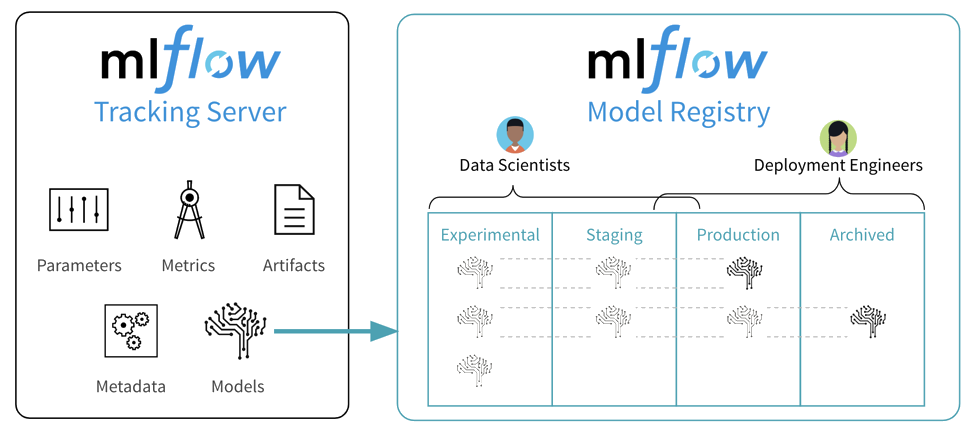
\includegraphics[width=\textwidth]{sections/img/mlflow-model-registry.png}}
    \caption{Core components of MLFlow. Source: Databricks.}
    \label{fig:mlflow-components}
\end{figure}






\subsection{Leveraging cloud technologies to foster iterative development}

While continuous improvement is a fundamental principle of MLOps, it is also a very demanding one. In particular, it requires to design and build our project as an integrated pipeline whose various stages are mainly automated, from data ingestion to monitoring the model in production. In this context, iterative development is essential in order to build a minimum viable product that is then refined over time. This section aims to show how cloud-native technologies, through the Onyxia project, were instrumental in building the project from the start as a collection of modular connected components, thus greatly enhancing the capacity for continuous refinement over time.

\subsubsection{A flexible development environment}

In a ML project, the flexibility of the development environment is essential. First, due to the diversity of tasks to be performed — data collection, preprocessing, modeling, evaluation, inference, monitoring, etc. Second, because ML is a fast-evolving field, it is preferable to build a ML app as a collection of modular components so as to be able to update components without disrupting the entire pipeline. As discussed in section~\ref{sec:cloud-native}, cloud-native technologies enable the creation of modular and scalable development environments.

However, as also discussed in section~\ref{sec:implementation}, access to such resources is not enough. A ML project that is developed following MLOps principles requires a wide variety of tools — data storage, interactive development environments to experiment freely, automation tools, monitoring tools, etc. While these tools can be installed on a Kubernetes cluster, making them available to data scientists in an integrated and pre-configured manner is essential to facilitate their adoption. Through its catalog of services and the automatic injection of configuration in the services, Onyxia enables building projects that rely on multiple cloud-native components that can communicate readily with each other.

The way model training was carried out for this project emphasizes the flexibility provided by Onyxia in the experimentation phase. All the code performing the training is written in Python in the context of a VSCode service. As personal S3 credentials are injected in each service at startup, the various users of the projects can interact directly with the training data stored on a S3 bucket on MinIO, Onyxia's default object storage solution. All experiments performed for the model selection phase are logged on a shared instance of MLFlow, which stores logged data on a PostgreSQL instance automatically launched on Kubernetes and artifacts (trained models and associated metadata) on MinIO. The model was trained using grid-search for hyperparameter tuning and evaluated through cross-validation, a combination that is known to provide a better evaluation of the generalization performance of the model but also requires a lot of computing resources, due to the combinatory nature of testing many hyperparameters combinations. In our case, we leveraged Argo Workflows, an open-source workflow engine designed to orchestrate parallel jobs on Kubernetes, each job being specified as an independent container. It then becomes straightforward to compare performances of the different trained models and select the best one using the comparison and visualization tools available in the UI of MLFlow. 

In summary, the training stage was made efficient and reproducible thanks to the use of numerous modularly connected components — a distinctive feature of cloud-native technologies — readily made available to data scientists by Onyxia.

\subsubsection{Deploying a model}

Once candidate models have been optimized, evaluated and a best-performing model has been selected, the next step is to make it available to the application end users. Simply providing the trained model as an artifact or even just the code to train the model is not a convenient way to serve it, as it assumes that users have the resources, infrastructure, and knowledge required for training it under the same conditions. The goal is therefore to make the model available in a simple and interoperable manner, in the sense that it should be possible to query it with various programming languages. Furthermore, it should be possible for other applications to query the model in a programmatic way. 

Against that background, we opted to serve the model through a REST API. This technology has become a standard way to serve ML models as they offer several benefits. First, they fit very well a cloud-oriented environment: similarly to the other components of our stack, it makes it possible to query the model using standard HTTP requests, which contributes to the modularity of the system. It also means that they are interoperable: as they rely on standards technologies for queries (HTTP requests) and responses (generally, a JSON-formatted string), they are mostly agnostic to the programming language used to request them. Finally, they offer great scalability because of their stateless design. As each request must contain all the information needed to understand and process the request, REST APIs can easily be duplicated on different machines to balance a challenging load — a process known as horizontal scaling.

To develop the API that serves the model, we used FastAPI\footnote{\url{https://fastapi.tiangolo.com}}, a fast and well-documented web framework for building APIs with Python. The API code and required software dependencies are encapsulated into a Docker image so that it can be deployed as a container on the Kubernetes cluster. An important benefit of using Kubernetes is the ability to scale the API — through the number of API pods effectively deployed — to the demand and provide automatic load-balancing. Upon startup, the API automatically retrieves the correct model from the MLflow model registry, which acts as a proxy from the actual artifact of the production model, stored on MinIO. Using a MLflow model enables to integrate the pre-processing step before each prediction to the API, greatly simplifying inference regardless of the ML framework used. This deployment process is summarized in Figure \ref{fig:api-datalab}.

\begin{figure}[htbp]
    \centering
    \makebox[\textwidth][c]{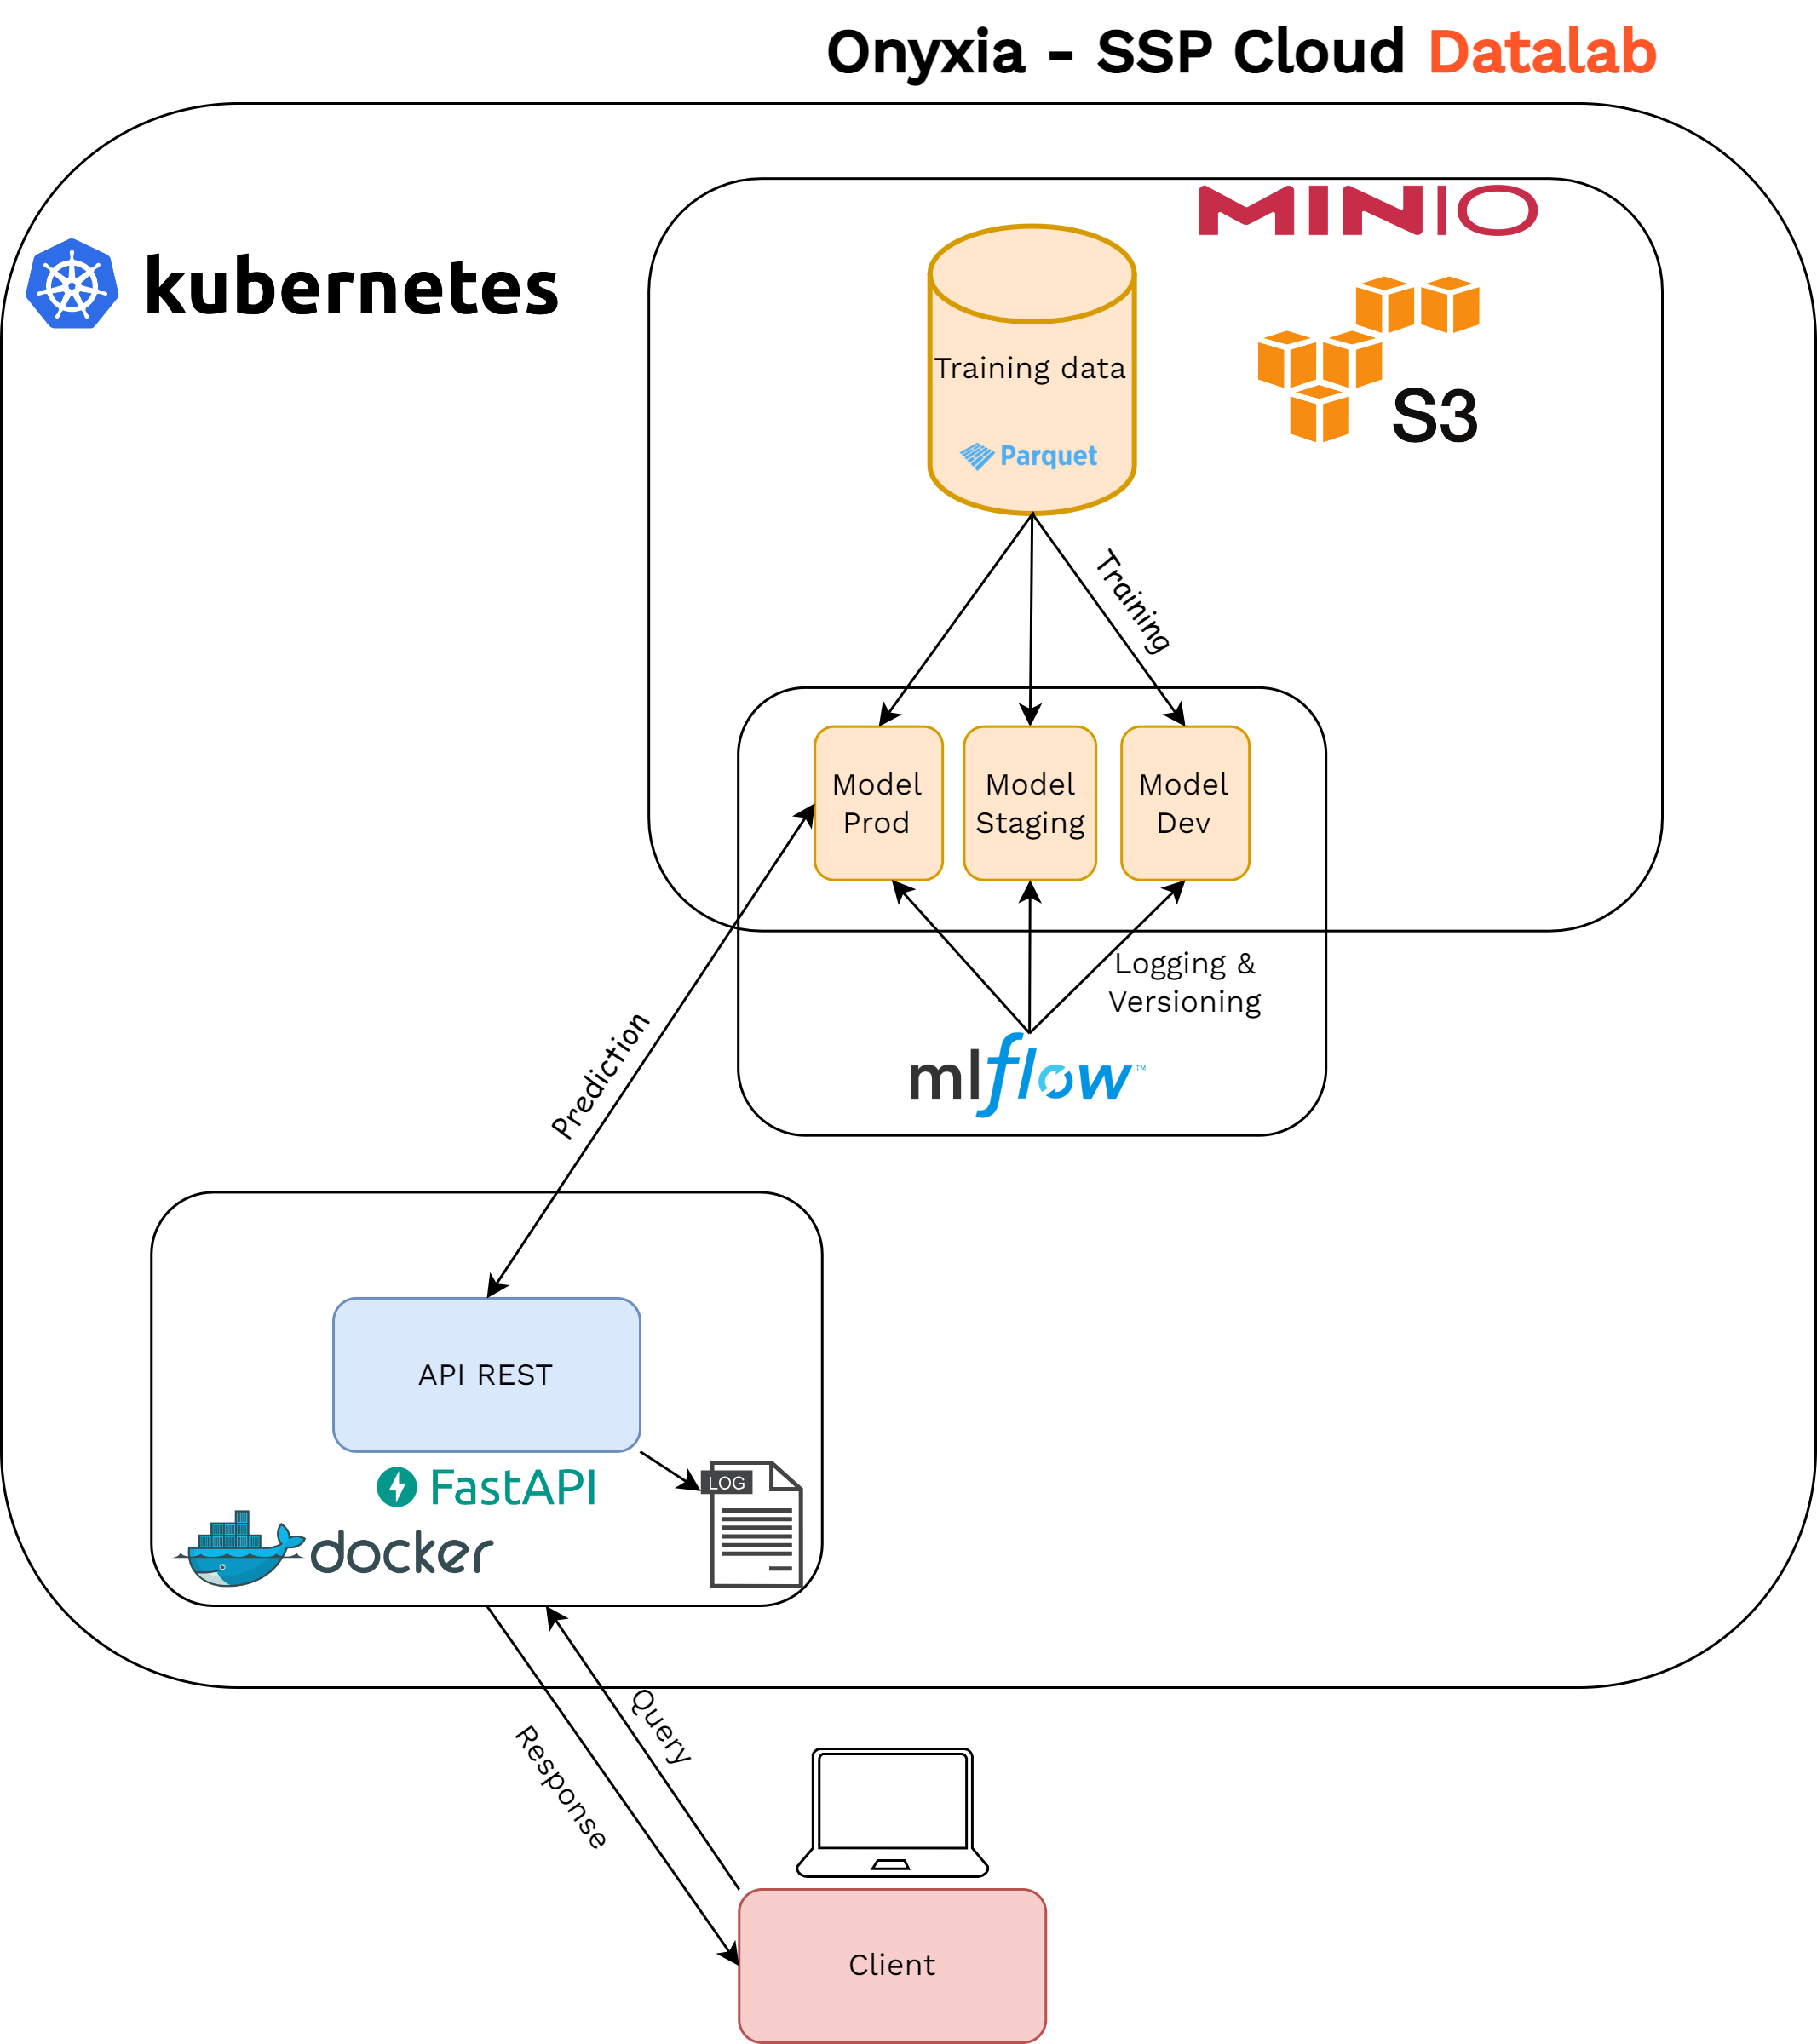
\includegraphics[width=0.75\textwidth]{sections/img/api-datalab.png}}
    \caption{A cloud-native approach to serve a ML Model using a REST API}
    \label{fig:api-datalab}
\end{figure}

\subsubsection{Building an integrated pipeline}

The architecture we built at this stage already reflects some important principles of MLOps. The use of containerization to deploy the API as well as the use of MLFlow to track the experiments while developing the model ensures reproducibility of the predictions. Using the central model registry provided by MLFlow facilitates the management of the lifecycle of the models in a collaborative way. Furthermore, the modularity of our architecture leaves room for further improvement as modular components can be easily added or modified without breaking the structure of the application as a whole. As we shall see in subsequent sections, this property was essential in building the application iteratively, enabling to add a monitoring layer (Section~\ref{subsubsec:monitoring}) and an annotation component (Section~\ref{subsubsec:annotation}) to promote continuous improvement of the model.

However, the ability to refine the base architecture iteratively also requires more continuity in the process. At this stage, the deployment process involves several manual operations. For instance, adding a new feature to the API would require to build a new image, tag it, update the Kubernetes manifests used to deploy the API and enforce them on the cluster to replace the existing one with minimum downtime. Similarly, a change of the model served through the API would require a very simple modification of the code but several manual steps to update the version on the cluster. As a result, data scientists are not fully autonomous when it comes to prototyping and testing updated versions of the model or the API, which limit the potential for continuous improvement.

In order to automate this process, we built a CI/CD pipeline — a concept already presented in Section~\ref{subsubsec:devops-mlops}) — integrating these various steps. Figure \ref{fig:ci-cd} illustrates our specific implementation of a CI/CD pipeline. Any change in the code of the API repository triggers a CI build process (implemented with GitHub Actions) of the associated docker image, which is then released on a public container registry (DockerHub). This image can then be fetched and deployed by the container orchestrator (Kubernetes), by specifying and applying manually new manifests to update the Kubernetes resources of the API. However, the downside of this approach is that it limits reproducibility of the deployment, since each resource is handled independently by the orchestrator, so that the lifecycle of the API deployment as a whole is not managed. To overcome this shortcoming, we integrate the deployment part in a CD pipeline based on the GitOps approach: the resources manifest of the API are stored on a Git repository. The state of this "GitOps" repository is monitored by a Kubernetes operator (ArgoCD), so that any change in the application manifests is directly propagated to the deployment on the cluster. In this integrated pipeline, the only action needed for the data scientist to trigger an update of the API is to change the tag of the API image indicating the version to be deployed.

\begin{figure}[htbp]
    \centering
    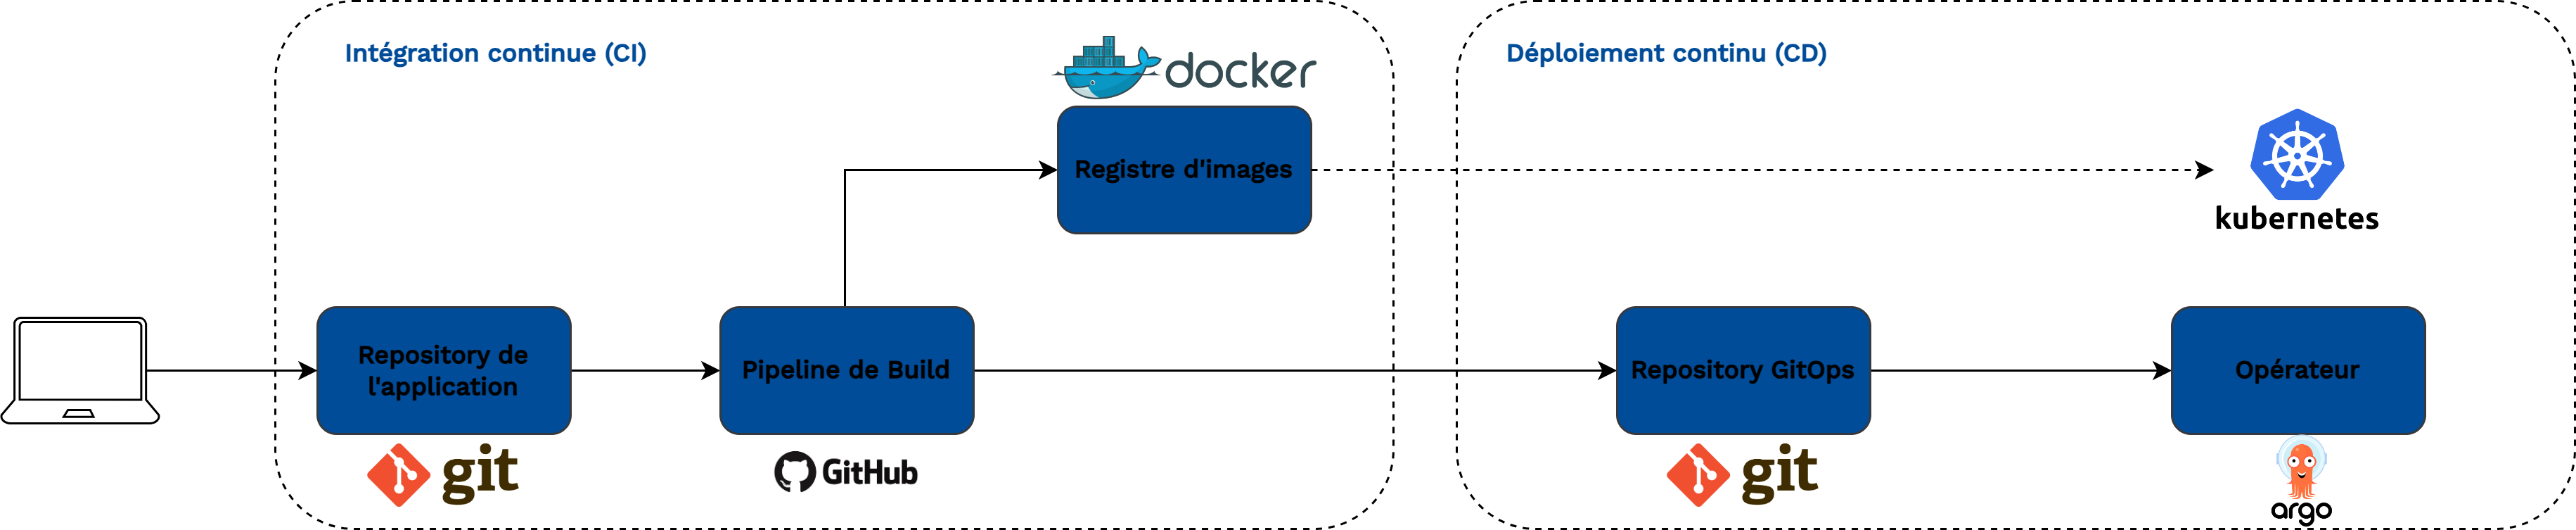
\includegraphics[width=\textwidth]{sections/img/ci-cd.png}
    \caption{The CI/CD pipeline implemented in the project}
    \label{fig:ci-cd}
\end{figure}

\subsubsection{Monitoring a model in production}
\label{subsubsec:monitoring}

Once the initial development phase of the project has been completed — including training, optimization, and deployment of the model to be served to users — it's crucial to understand that the data scientist's responsibilities extend further. Traditionally, the role of the data scientist is often limited to training the model and selecting the model to deploy, with the deployment task then delegated to the IT department. However, a specificity of ML projects is that, once in production, the model has not yet reached the end of its lifecycle, and it must be continuously monitored to prevent undesirable performance degradation. Continuous monitoring of the deployed model is extremely important to ensure the conformity of results to expectations, anticipate changes in data, and iteratively improve the model.

The concept of monitoring can take on different meanings depending on the context of the involved team. For IT teams, it primarily involves verifying the technical effectiveness of the application, including aspects such as latency, memory consumption, or disk usage. Conversely, for data scientists or business teams, the focus is more on methodological monitoring of the model. However, real-time tracking of the performance of a ML model is often a complex task, given that ground truth is usually not known at the time of prediction. Therefore, it is common to use proxies to detect any signs of performance degradation. Two main types of degradation of a ML model are generally distinguished:
\begin{itemize}
    \item \textbf{Data drift}: Data drift occurs when the data used during inference in production exhibits significant differences compared to the data used during training, that is,  $\mathds{P}_{train}(X) \neq \mathds{P}_{inference}(X)$ ;
    \item \textbf{Concept drift}: Concept drift is evoked when a change in the statistical relationship between the features ($X$) and the target variable ($Y$) is observed over time, that is, $\mathds{P}_{train}(Y|X) \neq \mathds{P}_{inference}(Y|X)$ and $\mathds{P}_{train}(X) = \mathds{P}_{inference}(X)$.
\end{itemize}

In the context of our project, the objective is to achieve the highest rate of correctly classified textual description while minimizing the number of textual description requiring manual intervention. Thus, our goal is to distinguish correct predictions from incorrect ones without prior access to ground truth. To accomplish this, we use a confidence index defined as the difference between the two highest confidence scores of the top results returned by the model. For a given textual description, if the confidence index exceeds a determined threshold, the textual description is automatically coded. Otherwise, the textual description is manually coded by an Insee's agent. This manual coding task is still informed by the ML model: through an application that queries the API, the agent is shown the five most probable codes according to the model. 

Defining the threshold for automatic coding of textual descriptions was thus crucial in this process, and involved making a trade-off between achieving a high automatic coding rate and maximizing coding performance. To monitor the behavior of our model in production, we developed an interactive dashboard that enables visualization of several metrics of interest for the business teams. Among these metrics are the number of requests per day and the rate of automatic coding per day based on a given confidence index threshold. This visualization allows business teams to understand the rate of automatic coding they would have obtained if they had chosen different thresholds. This dashboard also represents the distribution of obtained confidence indices and compare temporal windows in order to check for changes in the distributions of predictions returned by the model\footnote{Such distribution changes are typically checked by computing stastical distances — such as the Bhattacharyya distance, the Kullback-Leibler divergence, the Hellinger distance — and/or by performing statistical tests — such as the Kolmogorov–Smirnov or the chi-squared test.}. Finally, confidence indices can be analyzed at finer levels of granularity based on the aggregation level of the nomenclature, to determine which classes are most difficult to predict and which have more or less occurrences.

Figure \ref{fig:full-architecture} shows the components that were added to the project architecture so as to provide the monitoring dashboard described above. First, we set up a simple Extract-Transform-Load (ETL) process in Python (second box of the bottom row), which fetches the API logs periodically and transforms them into partitioned Parquet files. Then, we use the Quarto framework\footnote{Successor to R Markdown, Quarto has become an essential tool of our data stack. It unifies the functionality of several very useful packages from the R Markdown ecosystem while providing native support of several programming languages, including Python and Julia in addition to R. It is increasingly used at Insee as a way to produce reproducible documents and output them in a variety of formats.} to build an interactive dashboard (third box of the bottom row). To compute the various metrics presented in the dashboard, the Parquet files are queried using the SQL language through the DuckDB engine. Like the API, the dashboard is built and deployed as a container on the Kubernetes cluster, and this process is automated using a CI/CD pipeline. The annotation component (fourth box of the bottom row) is discussed in the next section.

\begin{figure}[htbp]
    \centering
    \makebox[\textwidth][c]{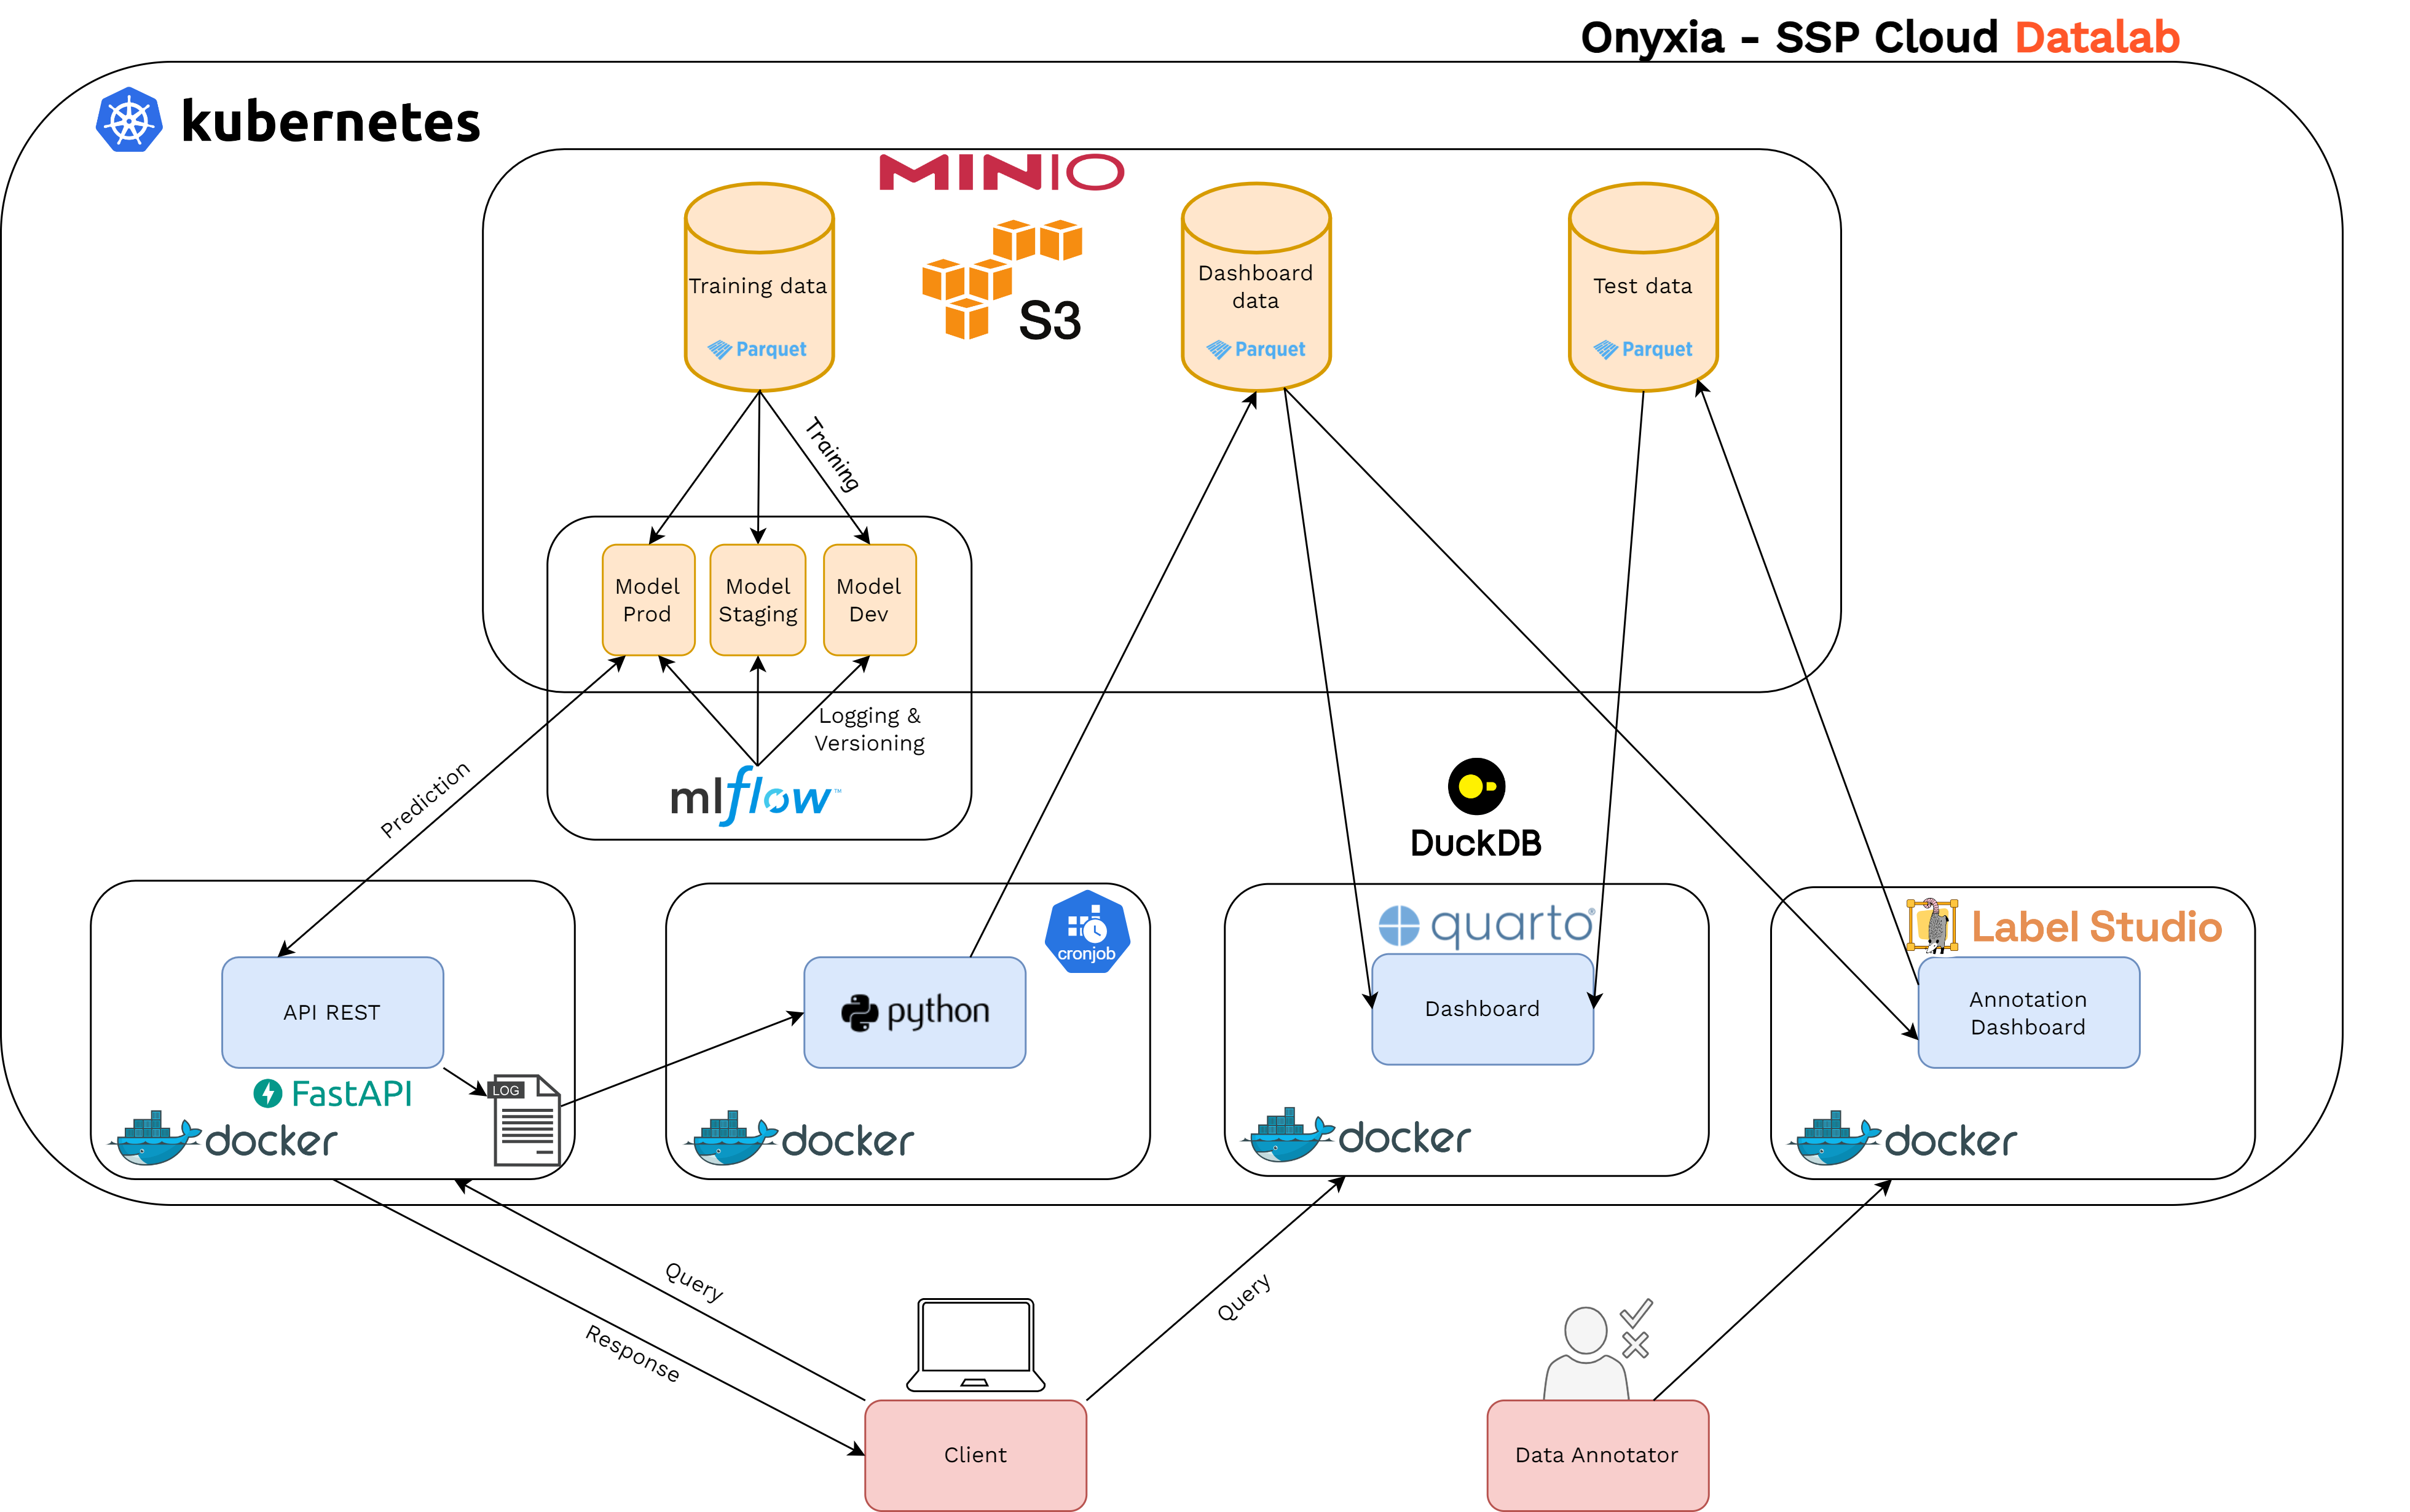
\includegraphics[width=1.5\textwidth]{sections/img/annotation-datalab.png}}
    \caption{Our implementation of a complete MLOps architecture}
    \label{fig:full-architecture}
\end{figure}

\subsubsection{Promoting continuous improvement of the model}
\label{subsubsec:annotation}

The monitoring layer of our application provides an important and detailed view into the system performance. Due to the dynamic nature of real-life data, ML models' performance often decline over time. To promote continuous improvement of the model, it is thus essential to envision strategies to overcome these performance losses. A frequently used strategy is periodic re-training of the model, which requires the collection of new training data.

After several months of the first version of the model running in production, the need to build a gold-standard test set became increasingly apparent. First, such a set was not accessible at the time of the experimentation phase, so we relied on a subset of the training dataset to perform evaluation, knowing the labeling quality was not optimal. Collecting a gold-standard sample would thus enable us to get an unbiased view of the model's performance in production on real data, particularly on data that has been automatically coded. Another reason is the redesign of the NACE nomenclature in 2025. From 2025 onwards, NSOs will be required to use the latest version of NACE, namely NACE Rev. 2.1. This revision brings substantial changes that will require an adaptation of the model, and thus the collection of new training set. Annotation of the old training dataset according to the new nomenclature is also considered to increase the size of the dataset.

Against that background, an annotation campaign has been initiated in early 2024 to build the new training set. The annotation campaign is carried out on the SSP Cloud using Label Studio, an open-source annotation tool that provides a user-friendly interface and is available in Onyxia's catalog. Figure \ref{fig:full-architecture} illustrates how the labelling component (fourth box of the bottom row) could be readily integrated in the project architecture thanks to its modular nature. In practice, we create a pool of text descriptions randomly sampled from the data passed through the API over the past three months. This sample is then sent to annotation by NACE experts using the UI of Label Studio. The annotation results are automatically saved on MinIO, transformed into Parquet format. Then, these gold-standard data are directly integrated into the monitoring dashboard to compute and observe various model performance metrics. These metrics give us a much clearer picture on the actual performance of the model on production data, and in particular on its shortcomings. This information will in turn be used to improve the model through periodical and targeted re-training in the near future. 
